%!TEX program = xelatex 
\documentclass{standalone}
\usepackage{pgfplots}
\usepackage{units}
\pgfplotsset{compat=1.8}% <-- moves axis labels near ticklabels
                        % (respects tick label widths)
\usepackage{tikz,tikz-3dplot}
\usetikzlibrary{arrows, positioning, calc, intersections, decorations.markings}

\begin{document}

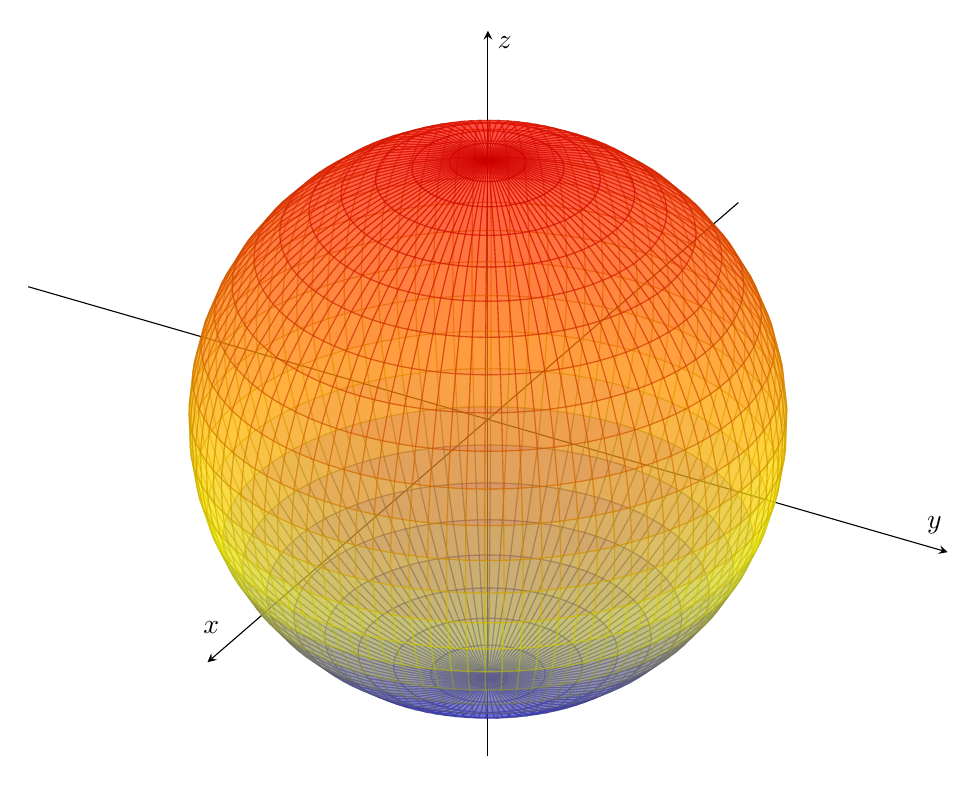
\begin{tikzpicture}
    \begin{axis}[%
        axis equal,
        width=20cm,
        height=20cm,
        axis lines = center,
        xmin=-1.3,xmax=1.5,ymin=-1.3,ymax=1.3,zmin=-1.3,zmax=1.5,
        xlabel=$x$,ylabel=$y$,zlabel=$z$,
        ticks=none,
        view={120}{30},
    ]
    \addplot3[%
        opacity = 0.5,
        surf,
        z buffer = sort,
        samples = 50,
        variable = \u,
        variable y = \v,
        domain = 0:180,
        y domain = 0:360,
    ]
    ({cos(u)*sin(v)}, {sin(u)*sin(v)}, {cos(v)});
    \end{axis}
\end{tikzpicture}

\end{document}